\documentclass[a4paper, 12pt]{article}
\usepackage[utf8]{inputenc}
\usepackage[english, russian]{babel}
\usepackage{amsmath}
\usepackage{tabularx}
\usepackage{graphicx}
\usepackage[left=2cm,right=2cm, top=2cm,bottom=2cm]{geometry}
\usepackage{tikz}

\begin{document}
\begin{flushright}
	Бавыкин Роман Р3110
\end{flushright}

\begin{center}
	Курсовая работа по дискретной математике. Часть 2\\
	\textbf{СИНТЕЗ МНОГОВЫХОДНЫХ КОМБИНАЦИОННЫХ СХЕМ}\\
	Вариант 2
\end{center}
$$C=\left|A-B\right|,\ A=(a_1,a_2,a_3),\ B=(b_1,b_2),\ C=(C_0,C_1,C_2)$$
\section{Составление таблицы истинности.}
\begin{tabularx}{0.9\textwidth}{
		| >{\centering\arraybackslash}X
		| >{\centering\arraybackslash}X
		| >{\centering\arraybackslash}X
		|| >{\centering\arraybackslash}X
		| >{\centering\arraybackslash}X
		|| >{\centering\arraybackslash}X
		| >{\centering\arraybackslash}X
		| >{\centering\arraybackslash}X|}
	\hline
	$a_1$ & $a_2$ & $a_3$ & $b_1$ & $b_2$ & $C_0$ & $C_1$ & $C_2$\\
	\hline
	\hline
	0 & 0 & 0 & 0 & 0 & 0 & 0 & 0\\
	\hline
	0 & 0 & 0 & 0 & 1 & 0 & 0 & 1\\
	\hline
	0 & 0 & 0 & 1 & 0 & 0 & 1 & 0\\
	\hline
	0 & 0 & 0 & 1 & 1 & 0 & 1 & 1\\
	\hline
	0 & 0 & 1 & 0 & 0 & 0 & 0 & 1\\
	\hline
	0 & 0 & 1 & 0 & 1 & 0 & 0 & 0\\
	\hline
	0 & 0 & 1 & 1 & 0 & 0 & 0 & 1\\
	\hline
	0 & 0 & 1 & 1 & 1 & 0 & 1 & 0\\
	\hline
	0 & 1 & 0 & 0 & 0 & 0 & 1 & 0\\
	\hline
	0 & 1 & 0 & 0 & 1 & 0 & 0 & 1\\
	\hline
	0 & 1 & 0 & 1 & 0 & 0 & 0 & 0\\
	\hline
	0 & 1 & 0 & 1 & 1 & 0 & 0 & 1\\
	\hline
	0 & 1 & 1 & 0 & 0 & 0 & 1 & 1\\
	\hline
	0 & 1 & 1 & 0 & 1 & 0 & 1 & 0\\
	\hline
	0 & 1 & 1 & 1 & 0 & 0 & 0 & 1\\
	\hline
	0 & 1 & 1 & 1 & 1 & 0 & 0 & 0\\
	\hline
	1 & 0 & 0 & 0 & 0 & 1 & 0 & 0\\
	\hline
	1 & 0 & 0 & 0 & 1 & 0 & 1 & 1\\
	\hline
	1 & 0 & 0 & 1 & 0 & 0 & 1 & 0\\
	\hline
	1 & 0 & 0 & 1 & 1 & 0 & 0 & 1\\
	\hline
	1 & 0 & 1 & 0 & 0 & 1 & 0 & 1\\
	\hline
	1 & 0 & 1 & 0 & 1 & 1 & 0 & 0\\
	\hline
	1 & 0 & 1 & 1 & 0 & 0 & 1 & 1\\
	\hline
	1 & 0 & 1 & 1 & 1 & 0 & 1 & 0\\
	\hline
	1 & 1 & 0 & 0 & 0 & 1 & 1 & 0\\
	\hline
	1 & 1 & 0 & 0 & 1 & 1 & 0 & 1\\
	\hline
	1 & 1 & 0 & 1 & 0 & 1 & 0 & 0\\
	\hline
	1 & 1 & 0 & 1 & 1 & 0 & 1 & 1\\
	\hline
	1 & 1 & 1 & 0 & 0 & 1 & 1 & 1\\
	\hline
	1 & 1 & 1 & 0 & 1 & 1 & 1 & 0\\
	\hline
	1 & 1 & 1 & 1 & 0 & 1 & 0 & 1\\
	\hline
	1 & 1 & 1 & 1 & 1 & 1 & 0 & 0\\
	\hline
\end{tabularx}
\newpage
\section{Минимизация булевых функций системы.}
\subsection*{$C_0$}
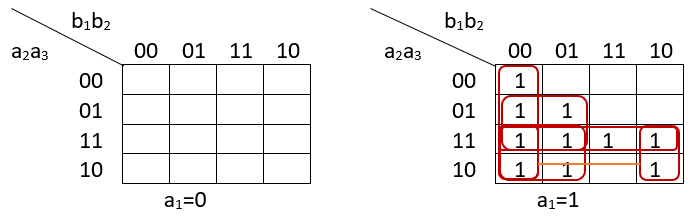
\includegraphics[width=14cm]{c0.png}\\

$C_{min}(C_0)=\left\lbrace
	\begin{array}{c}
		1XX00\\
		1X10X\\
		11X0X\\
		111XX\\
		11XX0
	\end{array}\right\rbrace,\
S^a=15,\ S^b=20$\\

$C_0={\mathstrut a}_1\bar{\mathstrut b}_1\bar{\mathstrut b}_2\vee
{\mathstrut a}_1{\mathstrut a}_3\bar{\mathstrut b}_1\vee
{\mathstrut a}_1{\mathstrut a}_2\bar{\mathstrut b}_1\vee
{\mathstrut a}_1{\mathstrut a}_2{\mathstrut a}_3\vee
{\mathstrut a}_1{\mathstrut a}_2\bar{\mathstrut b}_2$
\subsection*{$C_1$}
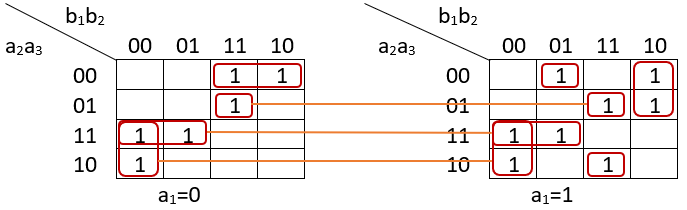
\includegraphics[width=14cm]{c1.png}\\

$C_{min}(C_1)=\left\lbrace
\begin{array}{c}
	X1X00\\
	X110X\\
	0001X\\
	10X10\\
	X0111\\
	00111\\
	10001
\end{array}\right\rbrace,\
S^a=28,\ S^b=35$\\

$C_1={\mathstrut a}_2\bar{\mathstrut b}_1\bar{\mathstrut b}_2\vee
{\mathstrut a}_2{\mathstrut a}_3\bar{\mathstrut b}_1\vee
\bar{\mathstrut a}_1\bar{\mathstrut a}_2\bar{\mathstrut a}_3{\mathstrut b}_1\vee
{\mathstrut a}_1\bar{\mathstrut a}_2{\mathstrut b}_1\bar{\mathstrut b}_2\vee
\bar{\mathstrut a}_2{\mathstrut a}_3{\mathstrut b}_1{\mathstrut b}_2\vee
\bar{\mathstrut a}_1\bar{\mathstrut a}_2{\mathstrut a}_3{\mathstrut b}_1{\mathstrut b}_2\vee
{\mathstrut a}_1\bar{\mathstrut a}_2\bar{\mathstrut a}_3\bar{\mathstrut b}_1{\mathstrut b}_2$
\subsection*{$C_2$}
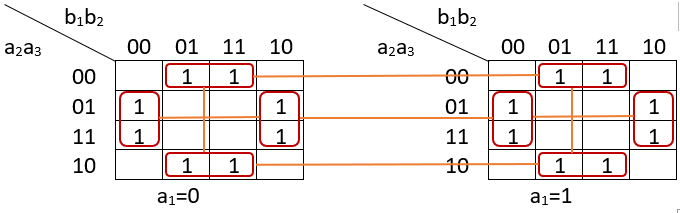
\includegraphics[width=14cm]{c2.png}\\

$C_{min}(C_1)=\left\lbrace
\begin{array}{c}
	XX0X1\\
	XX1X0
\end{array}\right\rbrace,\
S^a=4,\ S^b=6$\\

$C_2=\bar{\mathstrut a}_3{\mathstrut b}_2\vee
{\mathstrut a}_3\bar{\mathstrut b}_2$\\

$\left\lbrace\begin{array}{l r}
	C_0={\mathstrut a}_1\bar{\mathstrut b}_1\bar{\mathstrut b}_2\vee 
	{\mathstrut a}_1{\mathstrut a}_3\bar{\mathstrut b}_1\vee
	{\mathstrut a}_1{\mathstrut a}_2\bar{\mathstrut b}_1\vee
	{\mathstrut a}_1{\mathstrut a}_2{\mathstrut a}_3\vee
	{\mathstrut a}_1{\mathstrut a}_2\bar{\mathstrut b}_2, &
	\left(S_Q^{C_0}=20\right)\\\\
	
	C_1={\mathstrut a}_2\bar{\mathstrut b}_1\bar{\mathstrut b}_2\vee
	{\mathstrut a}_2{\mathstrut a}_3\bar{\mathstrut b}_1\vee
	\bar{\mathstrut a}_1\bar{\mathstrut a}_2\bar{\mathstrut a}_3{\mathstrut b}_1\vee
	{\mathstrut a}_1\bar{\mathstrut a}_2{\mathstrut b}_1\bar{\mathstrut b}_2\vee
	\bar{\mathstrut a}_2{\mathstrut a}_3{\mathstrut b}_1{\mathstrut b}_2\vee
	\bar{\mathstrut a}_1\bar{\mathstrut a}_2{\mathstrut a}_3{\mathstrut b}_1{\mathstrut b}_2\vee
	{\mathstrut a}_1\bar{\mathstrut a}_2\bar{\mathstrut a}_3\bar{\mathstrut b}_1{\mathstrut b}_2, &
	\left(S_Q^{C_1}=35\right)\\\\
	
	C_2=\bar{\mathstrut a}_3{\mathstrut b}_2\vee
	{\mathstrut a}_3\bar{\mathstrut b}_2. &
	\left(S_Q^{C_2}=6\right)
\end{array}\right.$\\

При реализации схемы в виде трех независимых подсхем ее цена $S_Q=61$.
\section{Преобразование минимальных форм булевых функций системы}

Решим задачу факторизации применительно к функциям $C_0$ и $C_1$.\\

$\left\lbrace\begin{array}{l r}
	C_0={\mathstrut a}_1\bar{\mathstrut b}_1\bar{\mathstrut b}_2\vee 
	{\mathstrut a}_1{\mathstrut a}_3\bar{\mathstrut b}_1\vee
	{\mathstrut a}_1{\mathstrut a}_2\bar{\mathstrut b}_1\vee
	{\mathstrut a}_1{\mathstrut a}_2{\mathstrut a}_3\vee
	{\mathstrut a}_1{\mathstrut a}_2\bar{\mathstrut b}_2=
	{\mathstrut a}_1\left(\left({\mathstrut a}_2\vee\bar{\mathstrut b}_1\right)
	\left({\mathstrut a}_3\vee\bar{\mathstrut b}_2\right)\vee
	{\mathstrut a}_2\bar{\mathstrut b}_1\right), &
	\left(S_Q^{C_0}=12\right)\\\\
	
	C_1={\mathstrut a}_2\bar{\mathstrut b}_1\bar{\mathstrut b}_2\vee
	{\mathstrut a}_2{\mathstrut a}_3\bar{\mathstrut b}_1\vee
	\bar{\mathstrut a}_1\bar{\mathstrut a}_2\bar{\mathstrut a}_3{\mathstrut b}_1\vee
	{\mathstrut a}_1\bar{\mathstrut a}_2{\mathstrut b}_1\bar{\mathstrut b}_2\vee
	\bar{\mathstrut a}_2{\mathstrut a}_3{\mathstrut b}_1{\mathstrut b}_2\vee
	\bar{\mathstrut a}_1\bar{\mathstrut a}_2{\mathstrut a}_3{\mathstrut b}_1{\mathstrut b}_2\vee
	{\mathstrut a}_1\bar{\mathstrut a}_2\bar{\mathstrut a}_3\bar{\mathstrut b}_1{\mathstrut b}_2, = & \\
	\quad\ ={\mathstrut a}_2\bar{\mathstrut b}_1\left({\mathstrut a}_3\vee
	\bar{\mathstrut b}_2\right)\vee\bar{\mathstrut a}_2{\mathstrut b}_1\left(
	\bar{\mathstrut a}_1\bar{\mathstrut a}_3\vee{\mathstrut a}_1\bar{\mathstrut b}_2\vee
	{\mathstrut a}_3{\mathstrut b}_2\vee\bar{\mathstrut a}_1{\mathstrut a}_3
	{\mathstrut b}_2\right)\vee{\mathstrut a}_1\bar{\mathstrut a}_2\bar{\mathstrut a}_3
	\bar{\mathstrut b}_1\bar{\mathstrut b}_2, & 
	\left(S_Q^{C_1}=29\right)\\\\
	
	C_2=\bar{\mathstrut a}_3{\mathstrut b}_2\vee
	{\mathstrut a}_3\bar{\mathstrut b}_2. &
	\left(S_Q^{C_2}=6\right)
\end{array}\right.$\\

За счет раздельной факторизации цена схемы уменьшилась: $S_Q=47$

Решим задачу факторизации применительно ко всем функциям системы, выделяя общие части и обозначая их как дополнительные функции:\\

$\left\lbrace\begin{array}{l r}
	z_1={\mathstrut a}_2\vee\bar{\mathstrut b}_1 & \left(S_Q^{z_1}=2\right)\\\\
	
	z_2={\mathstrut a}_3\vee\bar{\mathstrut b}_2 & \left(S_Q^{z_2}=2\right)\\\\
	
	z_3={\mathstrut a}_2\bar{\mathstrut b}_1 & \left(S_Q^{z_3}=2\right)\\\\
	
	z_4={\mathstrut a}_1\bar{\mathstrut b}_2 & \left(S_Q^{z_4}=2\right)\\\\
	
	C_0={\mathstrut a}_1\left({\mathstrut z}_1{\mathstrut z}_2\vee{\mathstrut z}_3\right) &
	\left(S_Q^{C_0}=6\right)\\\\
	
	C_1={\mathstrut z}_2{\mathstrut z}_3\vee\bar{\mathstrut z}_1\left(
	\bar{\mathstrut a}_1\bar{\mathstrut a}_3\vee{\mathstrut z}_4\vee
	{\mathstrut a}_3{\mathstrut b}_2\vee\bar{\mathstrut a}_1{\mathstrut a}_3
	{\mathstrut b}_2\right)\vee\bar{\mathstrut a}_2\bar{\mathstrut a}_3
	\bar{\mathstrut b}_1{\mathstrut z}_4, & 
	\left(S_Q^{C_1}=22\right)\\\\
	
	C_2=\bar{\mathstrut z}_2\vee{\mathstrut a}_3\bar{\mathstrut b}_2. &
	\left(S_Q^{C_2}=4\right)
\end{array}\right.$\\

После совместной факторизации цена схемы $S^Q=42.$
\section{Синтез многовыходной комбинационной схемы в булевом базисе}
\includegraphics[width=14cm]{scheme.jpg}\\

Задержка схемы: $T_{C_0}=4\tau,\ T_{C_1}=4\tau,\ T_{C_2}=3\tau,\ 
T=\max(T_{C_0}, T_{C_1},T_{C_2})=4\tau$
\section{Анализ многовыходной комбинационной схемы}

На схеме показано определение реакции схемы на входной набор (11111). Значение выходного набора (100) соответствует таблице истинности, что подтверждает корректность построенной схемы, по крайней мере, в отношении рассматриваемого набора.
\end{document}